\section{Physics Informed Neural Networks}
\label{ch1:sec4}

In this section we describe physics informed neural networks, abbreviated by PINNs, which are neural networks, introduced in \cite{RaissiPerdikarisKarniadakisPart1:2017}, that are trained to solve learning tasks while respecting any given law of physics described by general non-linear partial differential equations. PINNs enable the solution of a wide range of problems in computational science, represent a pioneering technology leading to the development of new classes of numerical solution methods for partial differential equations, and can be considered as a gridless alternative to traditional approaches and as a novel data-driven approach to model inversion and system identification \cite[p.~3]{RaissiPerdikarisKarniadakis:2019}. \\
Most of the physical laws that govern the dynamics of a system can be described by partial differential equations. For example, the Navier-Stokes equations are a set of partial differential equations derived from the conservation laws that describe the physics of many phenomena of scientific and engineering interest. They can be used to model the weather, ocean currents, water flow in a pipe and air flow around a wing. However, these equations cannot be solved exactly and therefore numerical methods must be used such as a finite volume method, where these equations must be solved while accounting for prior assumptions, linearization, and adequate time and space discretization. \\
As discussed in the previous section, machine learning methods with deep neural networks offer a promising way to approximate any function, therefore it is only logical to use them also for the approximation of the solution of differential equations. If one follows the classical approach, in which one trains a network purely by feeding it with data obtained, for example, from empirical tests of the underlying system, two problems arise. First, when analysing complex physical, biological or technical systems, the cost of data acquisition is often prohibitive and one is faced with the challenge of drawing conclusions and making decisions based on incomplete information. For the often resulting small amount of data, most of the modern machine learning methods are not robust enough and offer no convergence guarantee, which is why the task of training a network with a few high-dimensional input and output values seems naive. Second, neural networks do not in general take into account the physical properties underlying the system generated from the physical law, and the degree of approximation accuracy they provide still depends heavily on a careful specification of the problem geometry and the initial and boundary conditions. Without this prior information, the solution is not unique and may lose physical correctness. Exactly this prior information, such as the principal physical laws governing the time-dependent dynamics of a system, or some empirically validated rules or other expertise, can act as a control agent that restricts the space of admissible solutions to a manageable size, which leads to the idea of a physics informed neural network. This neural network type uses the governing physical equations in the training process, i.e. PINNs are designed to be trained to satisfy both, the given training data and the governing differential equations. In turn, encoding such structured information in a learning algorithm leads to an increase in the information content of the data which the algorithm encounters, so that it can move quickly towards the correct solution and generalize well, even when only a small data set is available, which is in some sense a key property of PINNs. Therefore, with some knowledge of the physical properties of the problem and some form of training data, PINNs can be used to find an optimal solution with high accuracy. Moreover, PINNs can be used for data-driven discovery of partial differential equations or system identification, which is concerned with finding parameters that describe best the observed data of a test of a system, \cite[pp.~1-2]{RaissiPerdikarisKarniadakisPart1:2017}. However, this is not relevant for this work and will therefore not be discussed. \\
We concentrate on the problem of computing data-driven approximate solutions to non-linear partial differential equations, by encoding explicitly the differential equation formulation in the neural network. We consider the following general form of a differential equation:
\begin{equation}
    \label{PINN PDE}
    \partial_t u(t,x) + \mathcal{H} \left[ u \right] (t, x) = 0, \quad x \in \Omega, \quad t \in \left[ 0, T \right], 
\end{equation}
where $u(t,x)$ is the latent solution of the corresponding system, $\partial_t u(t,x)$ is its derivative with respect to the time $t$ in the period $\left[ 0, T \right]$, $\mathcal{H} \left[ \cdot \right]$ is a non-linear differential operator, $x$ is an independent, possibly multi-dimensional variable, defined over the domain $\Omega \subset \mathbb{R}^{n}$. The structure of \cref{PINN PDE} covers a wide range of problems in mathematical physics, including conservation laws, diffusion processes, advection-diffusion reaction systems, and kinetic equations, \cite[p.~3]{RaissiPerdikarisKarniadakisPart1:2017}. \\
A distinction is made between discrete time and continuous time models for PINNs, depending on the type and arrangement of the available data. We focus on the latter. For this purpose let $f(x,t)$ be defined as the left-hand-side of \cref{PINN PDE}, i.e.
\begin{equation}
    \label{Residual Network}
    r(t,x) = \partial_t u(t,x) + \mathcal{H} \left[ u \right] (t, x).
\end{equation}
The main innovation of PINNs is that in \cref{Residual Network}, $u$ is approximated by a deep neural network and thus \cref{Residual Network} becomes a so-called residual network, which encodes the governing physical equations, takes the output of the neural network that approximates $u$ and computes a residual. This means that in the basic formulation of PINNs, two networks are combined: the surrogate network $u_\theta$, which approximates $u$ and therefore receives the same input parameters $(t,x)$, and the resulting residual network $r_\theta$, which emerges when $u_\theta$ is substituted into \cref{Residual Network}, i.e. $r_\theta(t,x) = \partial_t u_\theta (t,x) + \mathcal{H} \left[ u_\theta \right] (t, x)$. In principle, any type of neural network can be used for the surrogate network $u_\theta$. The most common are simple (fully-connected) deep feed-forward neural networks, see e.g. \cite{RaissiPerdikarisKarniadakis:2019}, \cite{BlechschmidtErnst:2021}, \cite{Markidis:2021}. The choice of the activation functions in each layer is critical for the performance of PINNs. As shown by \cite{MishraMolinaro:2021} PINNs require sufficiently smooth activation functions such as the sigmoid function, \cref{Sigmoid}, or the hyperbolic tangent function, \cref{TanH}. Non-smooth activation functions, such as ReLU, \cref{ReLU}, lead to non-convergent methods, i.e. in the limit of an infinite training dataset a well-trained PINN with ReLU-like activation functions, the solution does not converge to the exact solution of the differential equation, see \cite{MishraMolinaro:2021}. To obtain the residual network $r_\theta$ from the surrogate network $u_\theta$, one exploits recent developments in automatic differentiation - one of the most useful but perhaps underused techniques in scientific computing - to differentiate the neural network $u_\theta(t,x)$ with respect to its input values $t$ and $x$. The application of automatic differentiation to elegantly and efficiently formulate the derivative by time of the surrogate network $\partial_t u_\theta$ and the application of the operator $\mathcal{H} \left[ u_\theta \right] (t,x)$ in the residual network $r_\theta(t,x)$ is the main strength of PINNs. We note that the networks $u_\theta$ and $r_\theta$ share the same weights $W$ and biases $b$, but generally not the same activation functions, since in the residual network $r_\theta$ the derivatives of the activation functions of $u_\theta$ are generally considered. Since $r_\theta$ contains only $u_\theta$ as a neural network and no other network, $u_\theta$ and $r_\theta$ also have the same network topology, but the propagation of information through the neural networks is different. \\

\begin{figure}[H]
    \begin{center}
        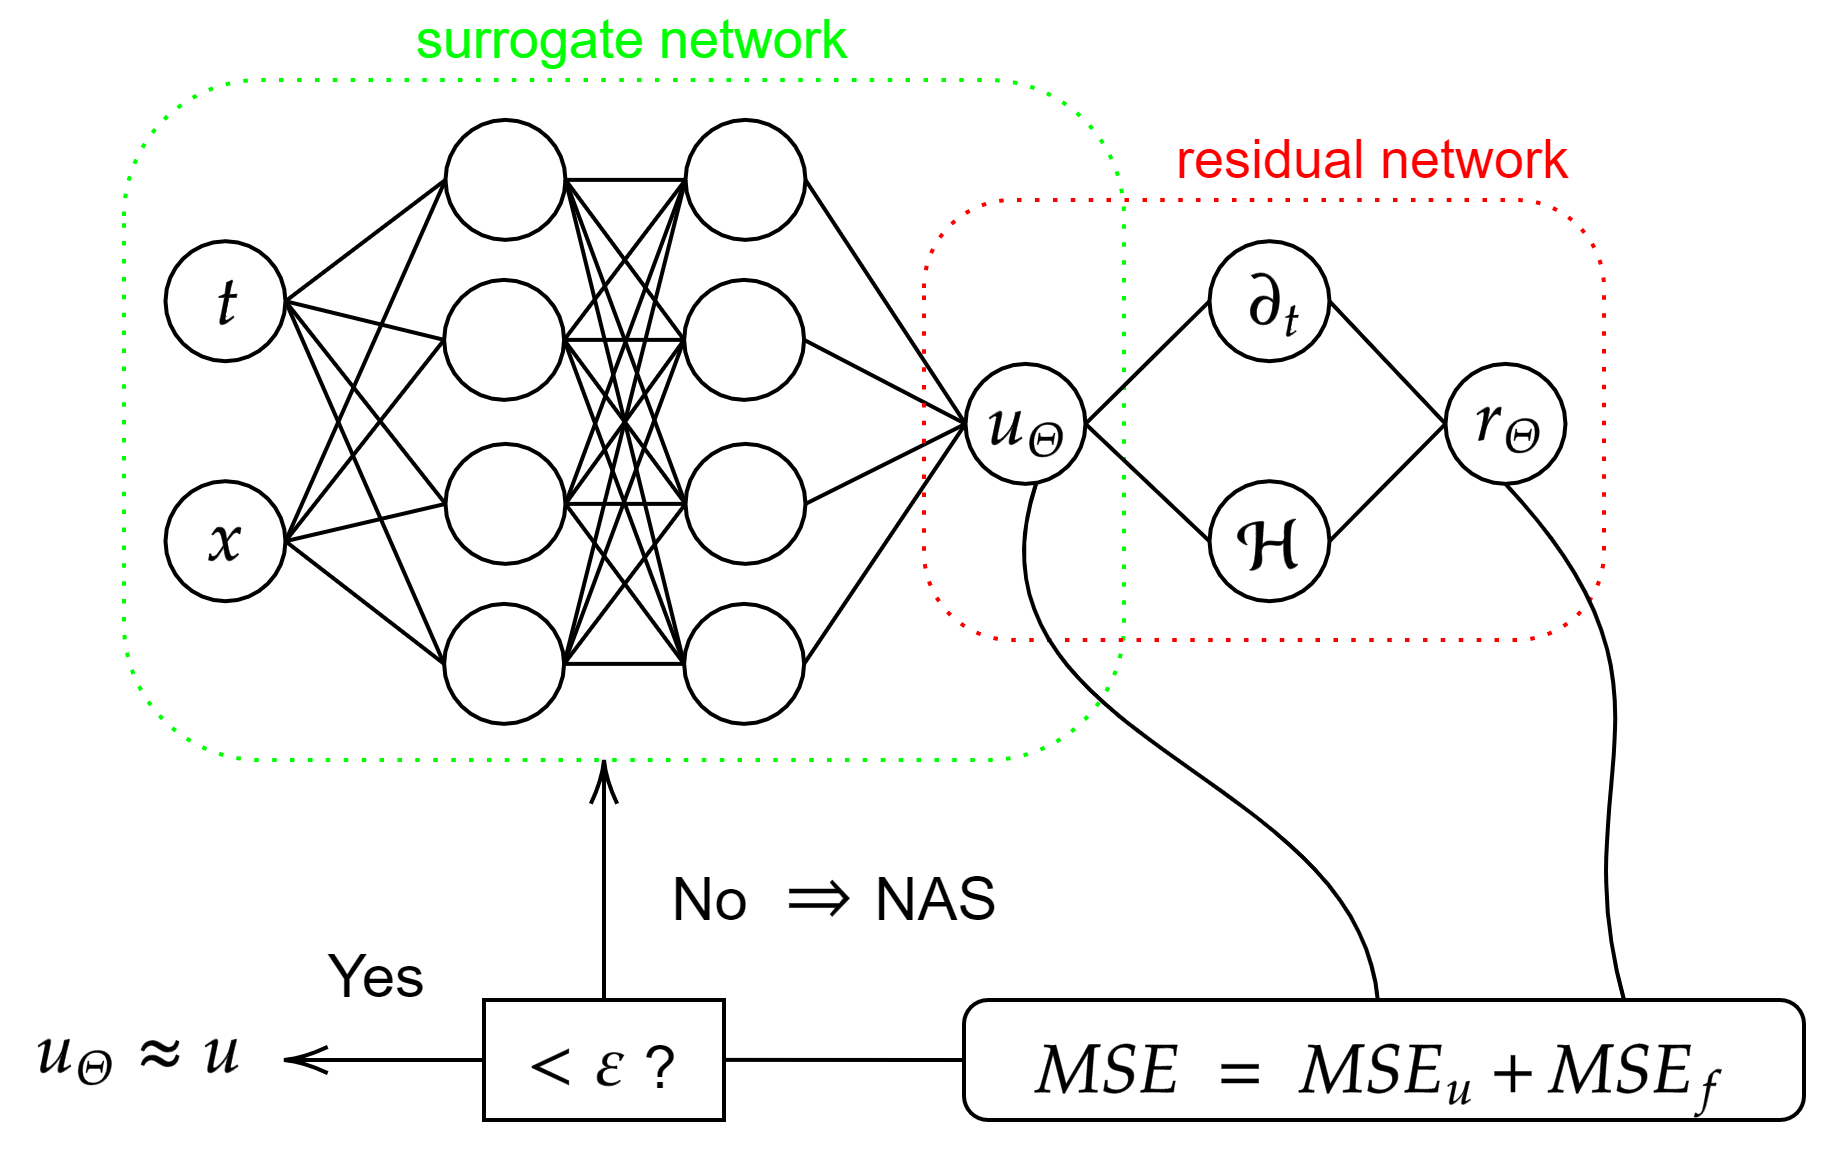
\includegraphics[scale=0.3]{img/diagram-20220212.png}
    \end{center}
    \caption{An illustration of a PINN to solve a problem with the governing differential equation \cref{PINN PDE}. The PINN consists of two basic interconnected networks. The first network (with green frame) illustrates the surrogate network $u_\theta(t,x)$, which should approximate the solution $u$ and therefore takes the same input. This network weights and biases are trainable. The second network (with red frame) illustrates the residual network $r_\theta(t,x)$, which takes the approximate solution from the surrogate network $u_\theta(t,x)$ and computes the residual using automatic differentiation. The residual $r_\theta(t,x)$ is used in a cost function to train the first network. The residual network includes the governing differential equation.}
    \label{fig6}
\end{figure}

PINNs are deep-learning networks that have to be trained. However, the residual network $r_\theta$, which is the characteristic feature of PINNs, is officially not trained, since its only function is to provide the surrogate network $u_\theta$ with the residual. The surrogate network $u_\theta$ of a PINN is trained, which afterwards returns an approximate solution $u_\theta$ of a differential equation for an input point $(t,x)$, which we call collocation point. The weights $W$ and biases $b$ of the surrogate network $u_\theta$ can be learned by minimizing the following cost function
\begin{equation}
    \label{MSE PINN}
    MSE = MSE_u + MSE_r, 
\end{equation}
where
\begin{equation*}
    MSE_u = \frac{1}{N_u} \sum^{N_u}_{i = 1} \lVert u_\theta(t^{u}_i, x^{u}_i) - u_i \rVert^{2}_{2}
\end{equation*}
and
\begin{equation*}
    MSE_r = \frac{1}{N_r} \sum^{N_r}_{i = 1} \lVert r_\theta (t^{r}_i, x^{r}_i) \rVert^{2}_{2}.
\end{equation*}
The data $\{t^{u}_i, x^{u}_i, u_i \}_{i = 1, \ldots, N_u}$ denotes the initial and boundary training data on $u_\theta$. It ensures with minimizing $MSE_u$ that $u_\theta$ takes over the initial and boundary conditions of the differential equation. The data is generated by using, for example, for $u_i$ the value $u(0,x^{u}_i)$ explicitly required by an initial condition for all points $x^{u}_i \in \Omega$, i.e. $t^{u}_i = 0$ for all $i = 1, \ldots, N_u$. With the collocation points $\{t^{r}_i, x^{r}_i \}_{i = 1, \ldots, N_r}$, the structured information imposed by the partial differential equation is to be enforced by $MSE_r$. We note that of course the value of $MSE$ also depends on both the size of the data sets, i.e. $N_u + N_r$, and the distribution of collocation points $\{t^{r}_i, x^{r}_i \}_{i = 1, \ldots, N_r}$ (with that $\{t^{u}_i, x^{u}_i \}_{i = 1, \ldots, N_u}$). One of the most used data set distributions is the uniform distribution, where the collocation points are uniformly spaced on $\left[ 0, T \right] \times \Omega$ as on a uniform grid. In addition, simulation or experimental data can also flow in for training the network in a supervised manner, which is for example necessary for data assimilation, inverse problems and super-resolution. We see that the learning of the network $u_\theta$, which is done by minimizing \cref{MSE PINN}, follows both a supervised approach through $MSE_u$ and an unsupervised approach through $MSE_r$. We nevertheless refer to the learning of PINNs as supervised learning, since both labelled data $u_i = u(t^{u}_i, x^{u}_i)$ is used in the optimization problem and by introducing $y_i=0$ for each collocation point $\{t^{r}_i, x^{r}_i \}_{i = 1, \ldots, N_r}$, we can form a supervised learning cost function from $MSE_r$. \\
In order to minimize $MSE$ in the training phase, two minimizers in succession are typically used: first an Adam optimizer which is an extended version of stochastic gradient descent method, see e.g. \cite{KingmaBa:2017}, and after that an L-BFGS-B optimizer, see e.g. \cite{ByrdLuNocedalZhu:1995}, which is a limited-memory version of the BFGS method to handle bound constrained optimization problems with many variables. Both methods only require the evaluation of $MSE$ and its gradient $\nabla_\theta MSE$ with respect to weights and biases. An L-BFGS-B method uses an approximation of the Hessian, which expresses the curvature of $MSE$ in the high-dimensional space of weights and biases, to determine the optimization direction and gives in general more accurate results. However, using an L-BFGS-B method directly without first using an Adam optimizer can quickly lead to a local minimum of $MSE$ without leaving it. Therefore, an Adam optimizer is used first to avoid local minima, and then the solution is refined by an L-BFGS-B method \cite[p.~6]{Markidis:2021}. \\
If the surrogate network $u_\theta$ has not been sufficiently trained by the available data so that it poorly approximates the solution $u$ of \cref{PINN PDE}, which can be seen by the amplitude of the value of $MSE$ (i.e. if the value of $MSE$ is very large, then $u_\theta$ approximates the solution $u$ in general poorly), then the choice of the topology or the activation functions or even the choice of the type of neural network should be reconsidered. This again belongs to the task area of the NAS or the hyperparameter optimization. After a PINN is trained successfully (this can be measured by $MSE < \varepsilon$, for example), the surrogate network $u_\theta$ can predict an approximate solution $u_\theta (t,x)$ to the governing differential equation \cref{PINN PDE} for each point $(t,x) \in \left[ 0, T \right] \times \Omega$. Thus, it is a gridless method as any point can be taken without the need to define a grid. Moreover, the trained surrogate network $u_\theta$ can be used to predict values on grids with different resolutions without having to be re-trained. For this reason, the computational cost does not depend on the number of grid points as in many traditional computational methods \cite[p.~2]{Markidis:2021}. \\
Although the idea of PINNs is still quite young, there are already several PINN frameworks with different network architectures for different PDE solutions. For example, \lstinline!fPINN! (fractional PINN), see \cite{PangLuKarniadakis:2019}, where the residual network is able to compute the residuals of the governing equations including fractional calculus operators, or \lstinline!vPINN! (variational PINN), see \cite{KharazmiZhangKarniadakis:2019}, where the residual network incorporates the variational form of the problem into the loss function \cite[pp.~5-6]{Markidis:2021}. All major PINN frameworks are written in \lstinline!Python!, \cite{Python}, and are based on either \lstinline!TensorFlow!, \cite{TensorFlow}, or \lstinline!PyTorch!, \cite{PyTorch}, to express the neural network architecture and to use automatic differentiation for defining the residual network \cite[p.~6]{Markidis:2021}. 

% Wir machen forward problem
% cPINN Paper nochmal anschauen
% Mehr Refs einfügen